\section{Comparison of models}\label{sec:evaluation-models}

% parameters
Similar to \citeauthor{glove2014}'s work, in this work, for many models used, any unspecified parameters are set to their default values, 
assuming that they are close to optimal
acknowledging that this simplification should be revised in a more thorough analysis.

% comparing models (qualitative)
This evaluation does not aim to find the best model but to compare the similarity of the models' query results.
The different query responses of the models are compared on a selection of documents.
The selection is obtained by randomly choosing \textcolor{red}{TODO: X} documents from a corpus of 2048 documents.
The 2048 document corpus was randomly chosen (without replacement) from the Bahamas leak.
The \textcolor{red}{TODO: Y} most similar documents for each selected document are retrieved from the database for each model and stored in a \ac{csv} file.
To facilitate working with the data, the document IDs can be encoded as monotonically increasing integers.

Furthermore, the query results are compared using a Venn diagram and a heatmap presented in \autoref{fig:comparison-models}.
% Venn diagram
To build a Venn diagram, the number of documents which are shared between the query results of two models is computed.
Hence, all query results of a model are saved in a set and the intersection of two sets is computed.
Since there are five models the Venn diagram consists of five circles.
It is possible to compare not only two but more models at once.
One should be cautious when interpreting the layout of the Venn diagram since 
an intersection of documents which produces an empty set has a non-empty area in this visualization.
\textcolor{red}{results derived from diagram}

% heatmap
Before the heatmap can be created, the shared query results of each model pair are computed and stored in a matrix.
The matrix consists of five rows and five columns, where each row and column represents a model.
The code snippet in \lst{lst:sim-matrix} shows the calculation of the similarity matrix.
The cell values are the number of shared query results between the models of the row and column.
They are calculated by summing up the number of shared query results per document query.
Since the matrix is symmetric, only the upper triangular matrix is computed and the other half is mirrored.
The matrix is then visualized using a heatmap.
\textcolor{red}{results derived from diagram}

\begin{listing}[htp]
    \begin{minted}{python3}
        sim_matr = np.matrix(np.zeros((len(model_names), len(model_names))))
        for id in df.index:
            for i, model in enumerate(model_names):
                for j in range(i, len(model_names)):
                    sim_matr[i, j] += np.sum([df.loc[id, 
                        model_names[j]].count(item) for item in df.loc[id, model]])
                    sim_matr[j, i] = sim_matr[i, j]
    \end{minted}
    \caption{Calculation of the similarity matrix used to produce the heatmap.
    }
    \label{lst:sim-matrix}
\end{listing}

\begin{figure}%
    \centering
    \subfloat[\centering Venn diagram of query results.]{{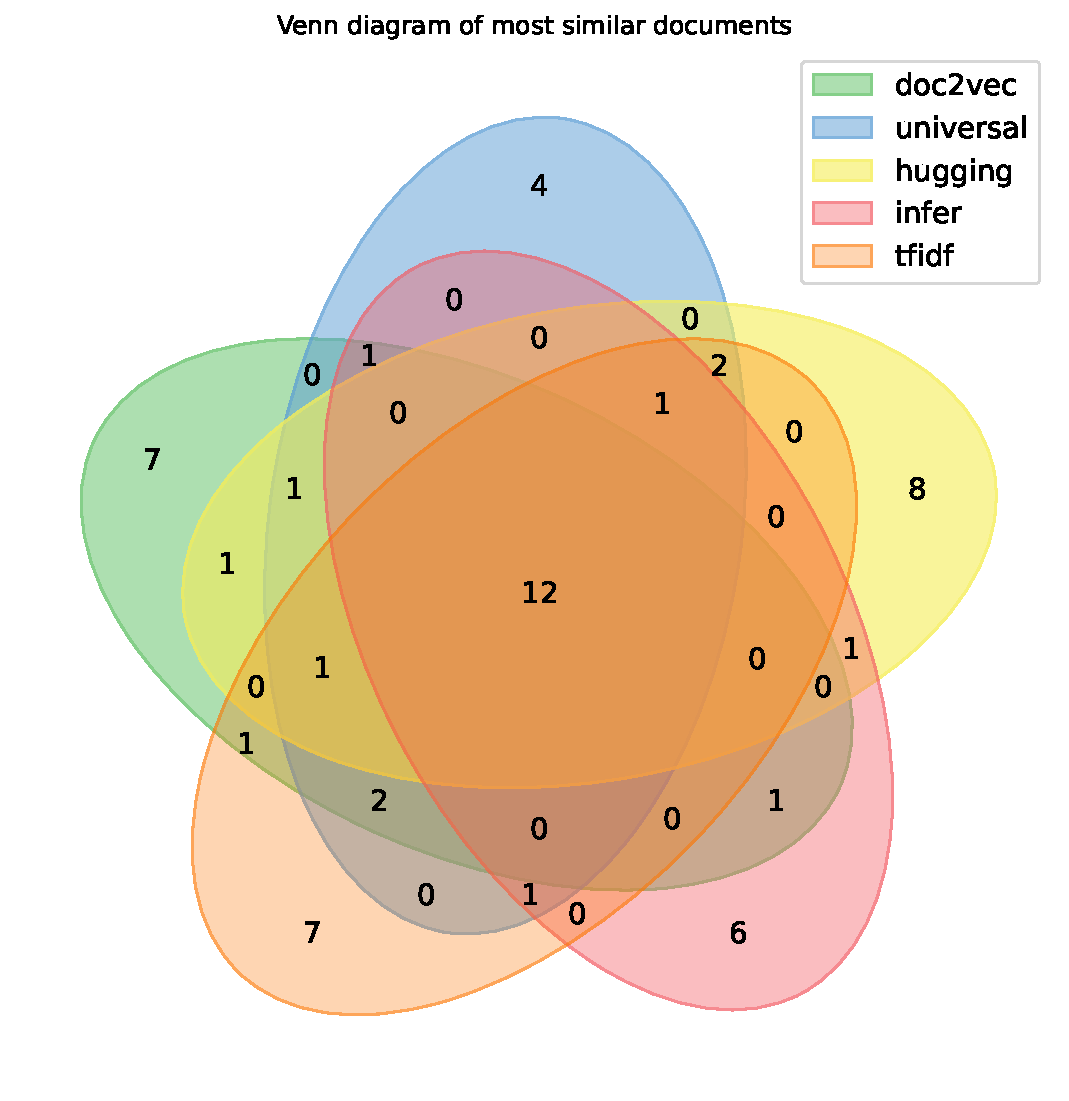
\includegraphics[width=4cm]{images/comparison/Venn_diagram_of_most_similar_documents.pdf} }}%
    \qquad
    \subfloat[\centering Heatmap visualizing shared query results.]{{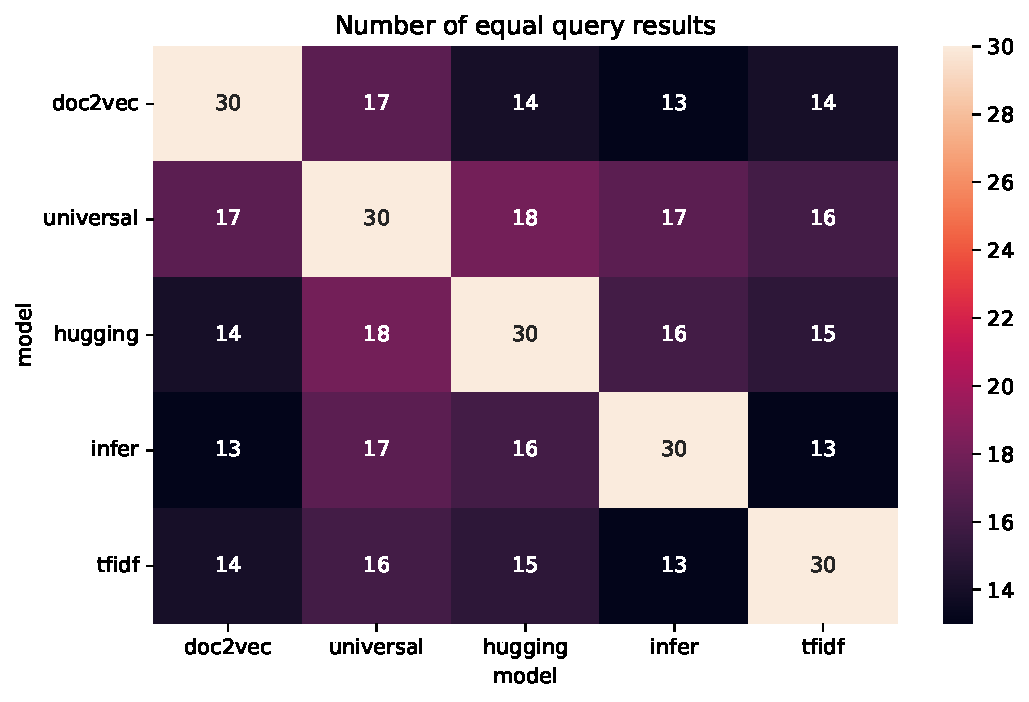
\includegraphics[width=6cm]{images/comparison/Number_of_equal_query_results.pdf} }}%
    \caption[Comparison of models]{Comparison of the results obtained by different models.}%
    \label{fig:comparison-models}%
\end{figure}


% sample query
To display the differences between the models exemplary, the five most similar docuemnts to a random document were returned from the database and visualized.
The text of the query document was encoded using the respective model and \ac{knn} query was used to obtain the results from the local database containing 2048 documents.
The query image was omitted from the database query response.
\autoref{fig:query_resp_doc2vec} displays \ac{d2v} reponses, ... 
\autoref{fig:query_resp_sbert}
\autoref{fig:query_resp_tfidf}
\autoref{fig:query_resp_infer}
\autoref{fig:query_resp_use}

% sample query
\begin{figure}[h!]
    \begin{subfigure}{\textwidth}
        \centering
        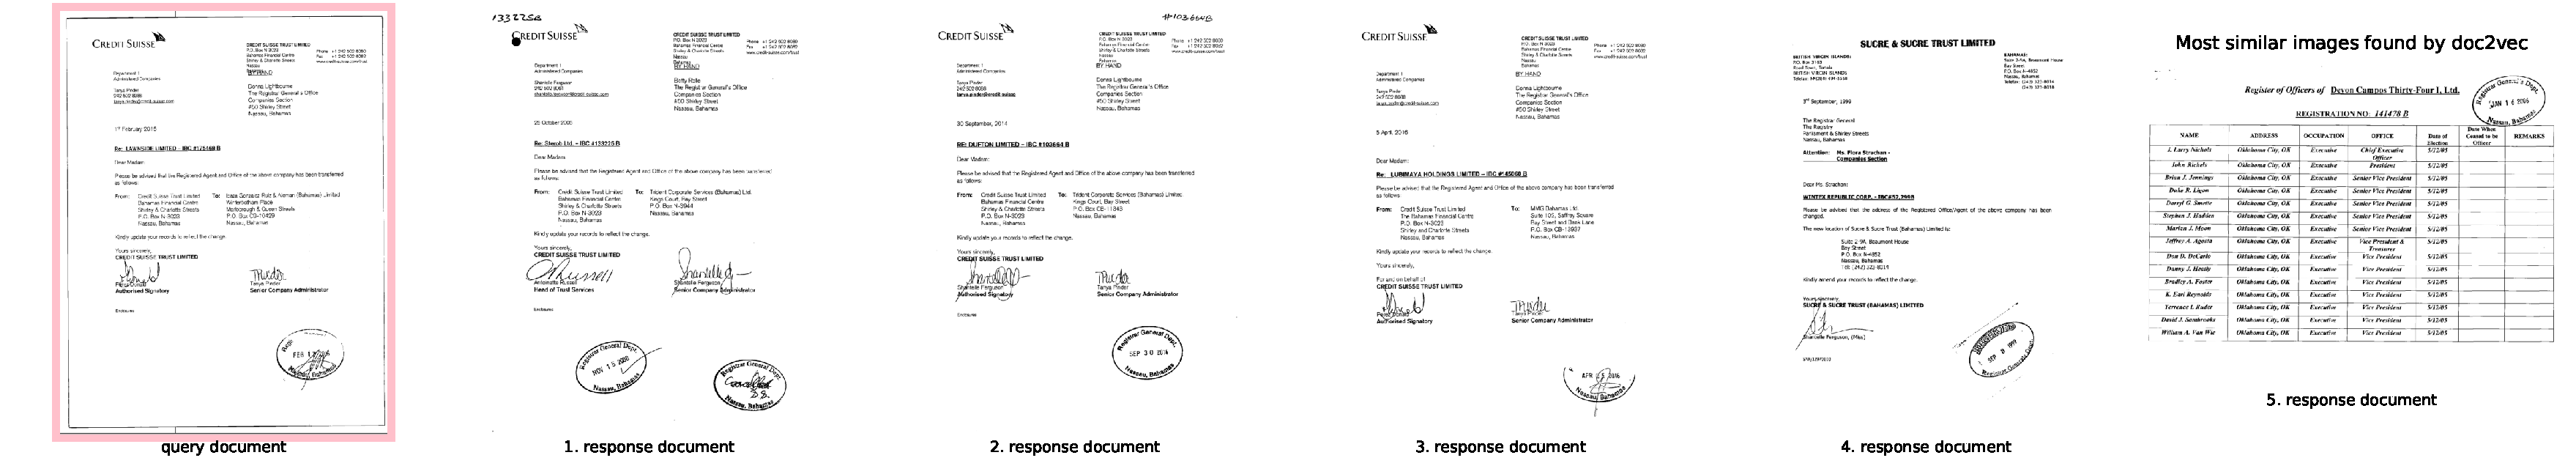
\includegraphics[width=1\textwidth]{images/query_results/4b4d0a9ee0c7283e5bfd69c402c73b2140bf90351c8f44d6809afe23c6dfaa50/Most_similar_images_found_by_doc2vec.pdf}
        \caption{\ac{d2v}}
        \label{fig:query_resp_doc2vec}
    \end{subfigure}

    \begin{subfigure}{\textwidth}
        \centering
        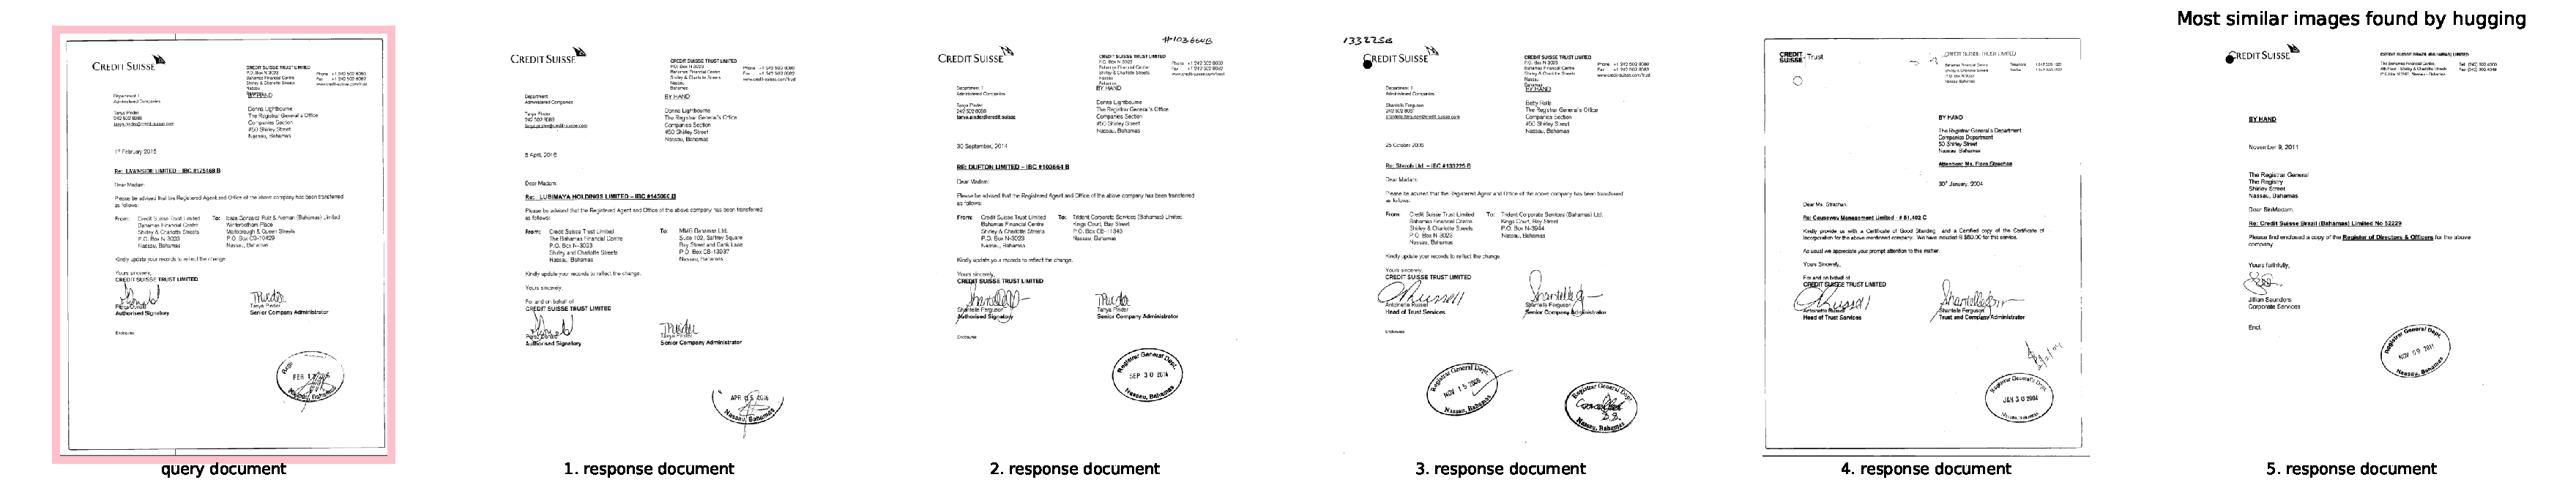
\includegraphics[width=1\textwidth]{images/query_results/4b4d0a9ee0c7283e5bfd69c402c73b2140bf90351c8f44d6809afe23c6dfaa50/Most_similar_images_found_by_hugging.pdf}
        \caption{\ac{sbert}}
        \label{fig:query_resp_sbert}
    \end{subfigure}

    \begin{subfigure}{\textwidth}
        \centering
        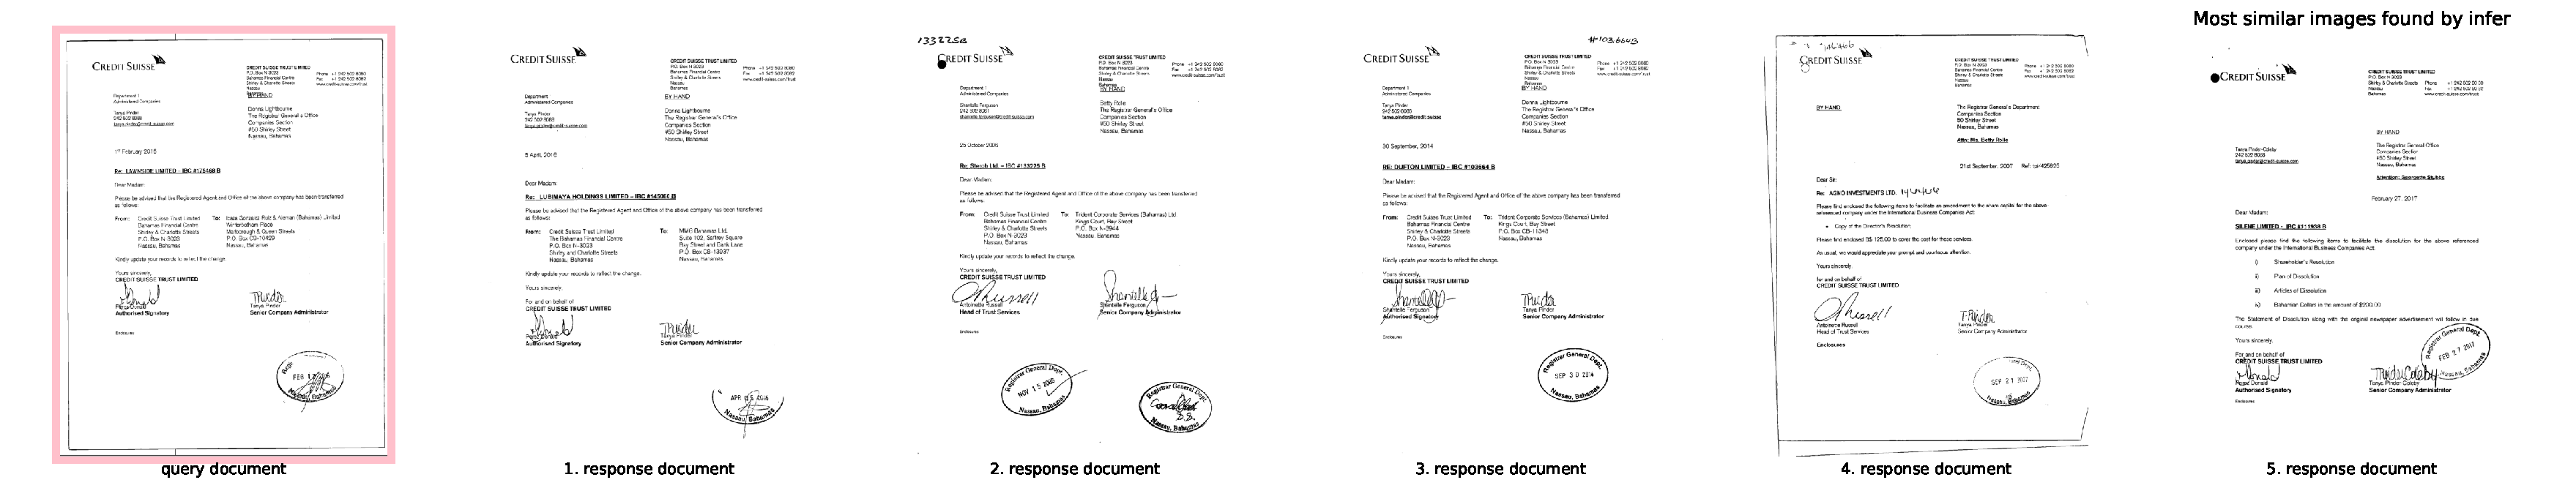
\includegraphics[width=1\textwidth]{images/query_results/4b4d0a9ee0c7283e5bfd69c402c73b2140bf90351c8f44d6809afe23c6dfaa50/Most_similar_images_found_by_infer.pdf}
        \caption{\infersent{}}
        \label{fig:query_resp_infer}
    \end{subfigure}

    \begin{subfigure}{\textwidth}
        \centering
        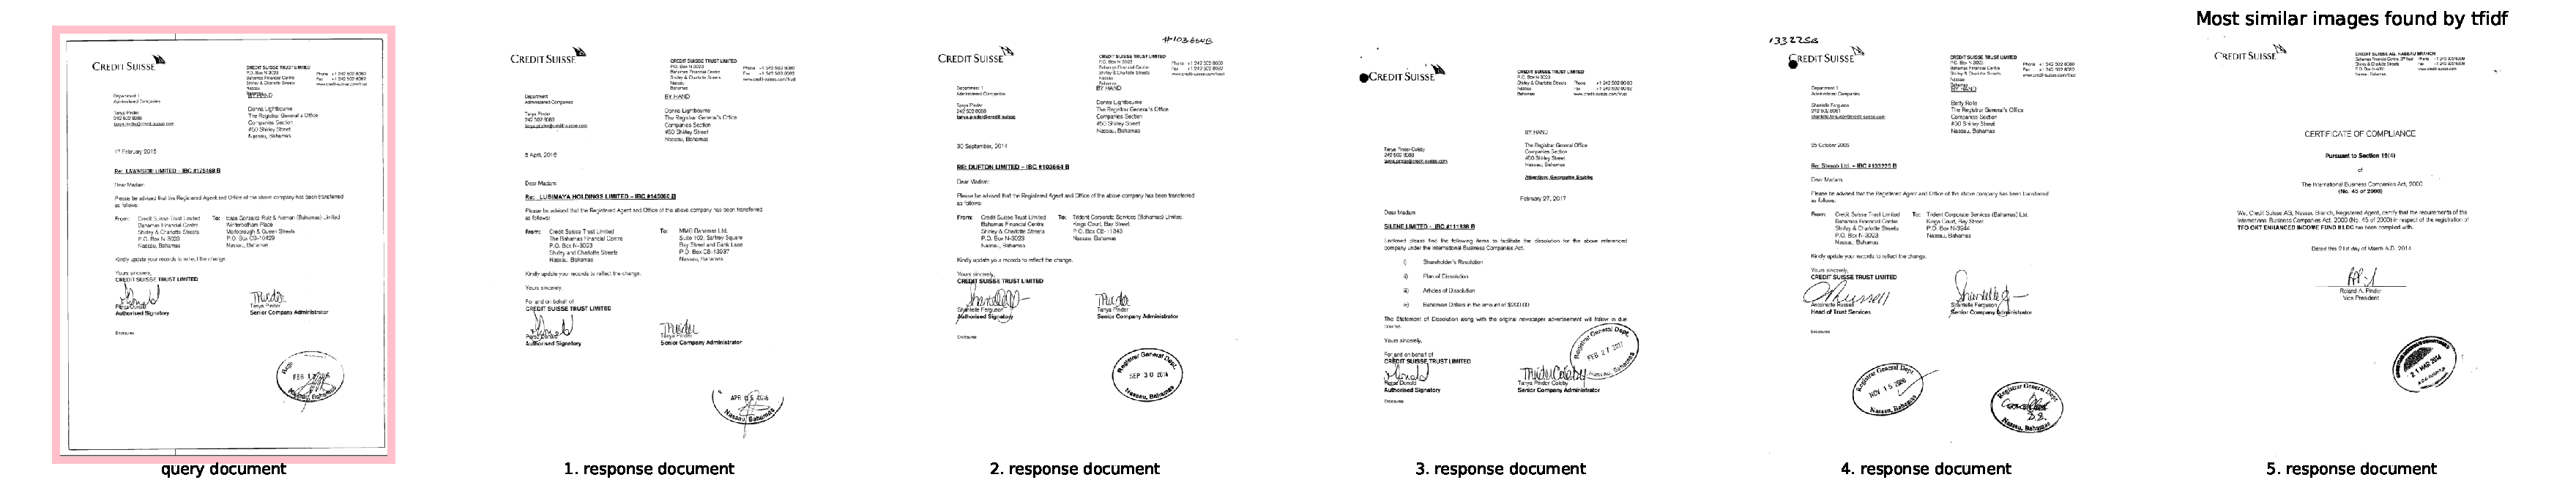
\includegraphics[width=1\textwidth]{images/query_results/4b4d0a9ee0c7283e5bfd69c402c73b2140bf90351c8f44d6809afe23c6dfaa50/Most_similar_images_found_by_tfidf.pdf}
        \caption{\ac{tfidf}}
        \label{fig:query_resp_tfidf}
    \end{subfigure}

    \begin{subfigure}{\textwidth}
        \centering
        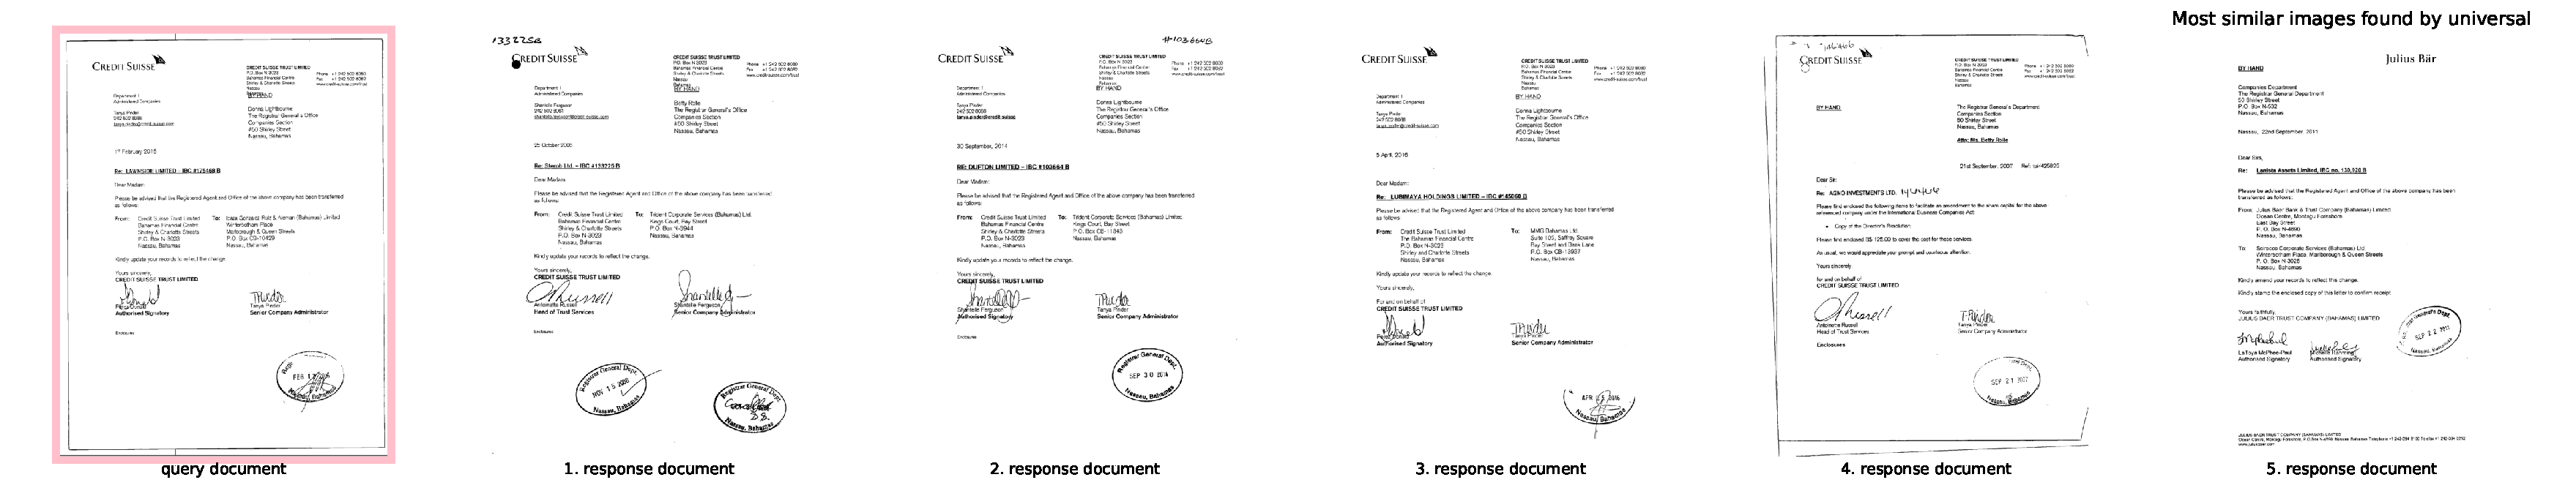
\includegraphics[width=1\textwidth]{images/query_results/4b4d0a9ee0c7283e5bfd69c402c73b2140bf90351c8f44d6809afe23c6dfaa50/Most_similar_images_found_by_universal.pdf}
        \caption{\ac{use}}
        \label{fig:query_resp_use}
    \end{subfigure}
\caption[Exemplary query response]{Exemplary query response in terms of similarity on different embeddings.}
\label{fig:query_resp}
\end{figure}

% good results
\begin{figure}[htp] % htp = hier (h), top (t), oder auf einer eigenen Seite (p).
    \centering
    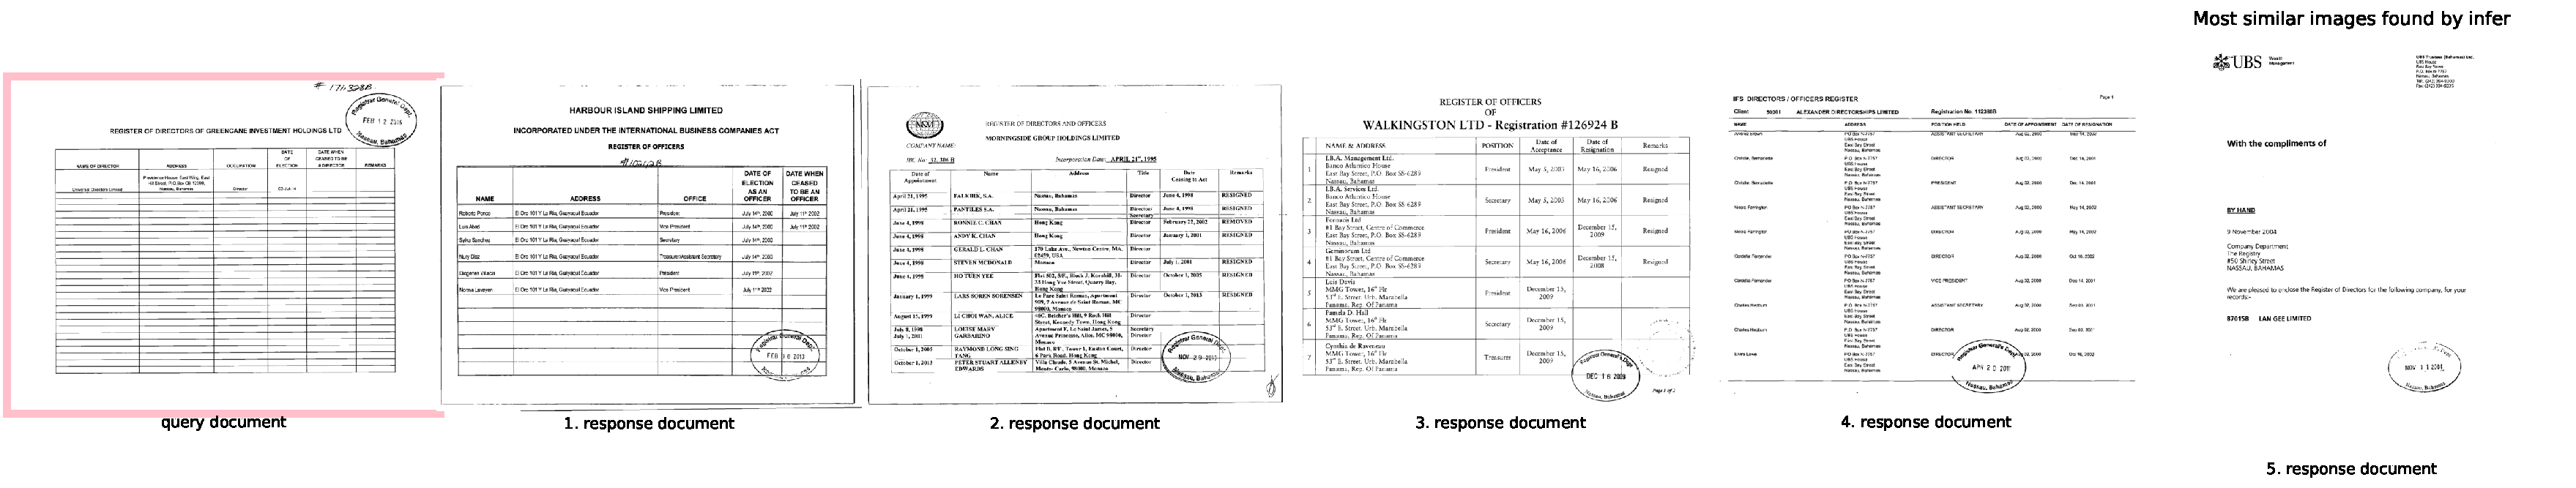
\includegraphics[width=1\textwidth]{images/query_results/42b7e56855c88c22ed01f381167e6f0887815e1ef7ea6b149be06ee1f8557b9e/Most_similar_images_found_by_infer.pdf}
    \caption[\infersent{} query responses]{\infersent{} query responses on a query document consisting of little text.
    }
    \label{fig:good_query_resp_infer}
\end{figure}

% bad results
\begin{figure}[h!]
    \ContinuedFloat
    \begin{subfigure}{\textwidth}
        \centering
        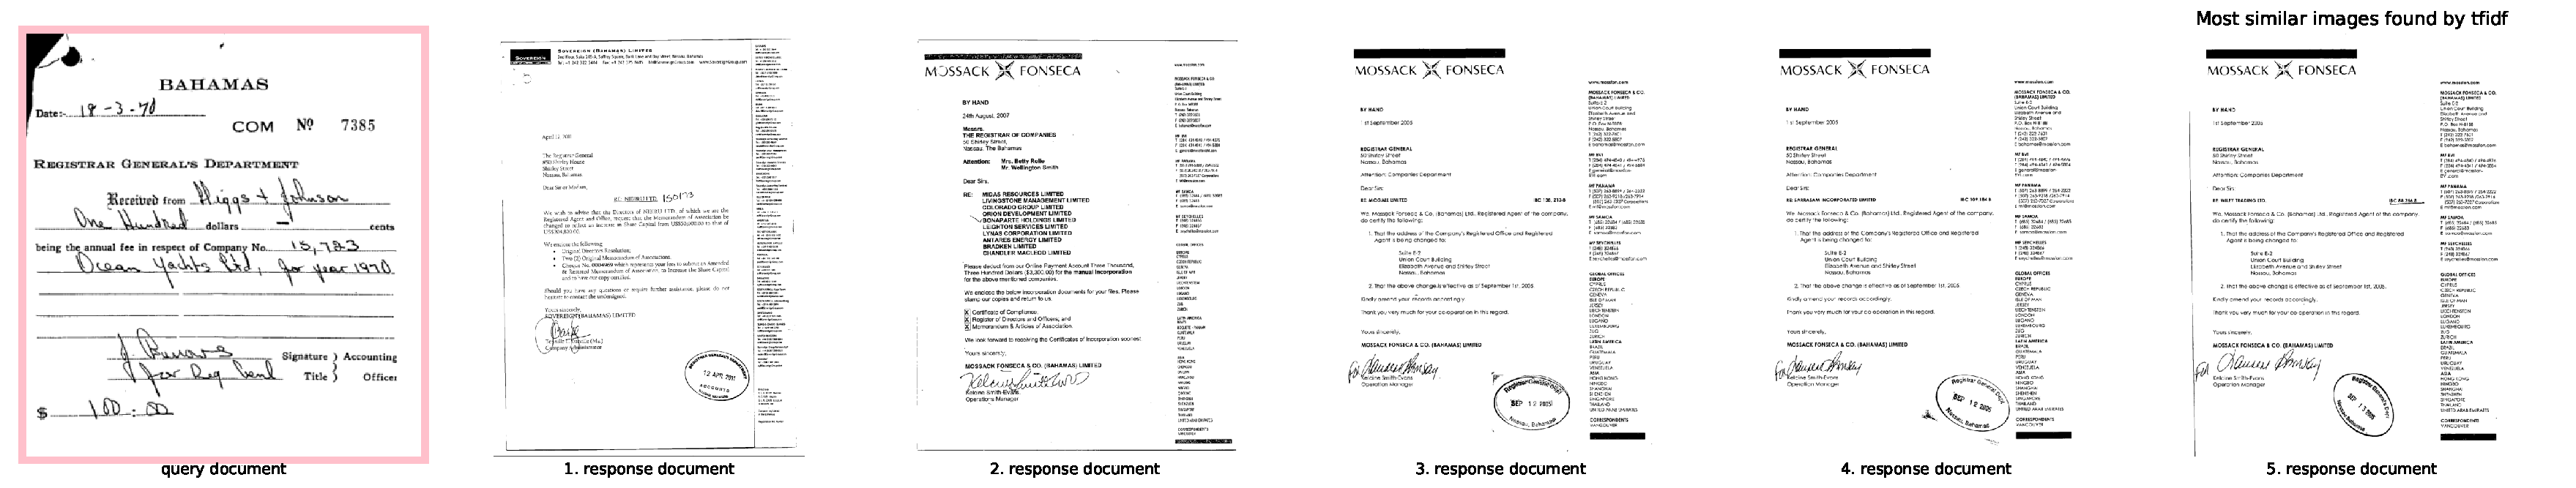
\includegraphics[width=1\textwidth]{images/query_results/4542b223317eba23e4bda3e1536d61c8e2d2890a6439830ca8c62650bc1aac70/Most_similar_images_found_by_tfidf.pdf}
        \caption{\ac{tfidf}}
        \label{fig:bas_query_resp_tfidf}
    \end{subfigure}

    \begin{subfigure}{\textwidth}
        \centering
        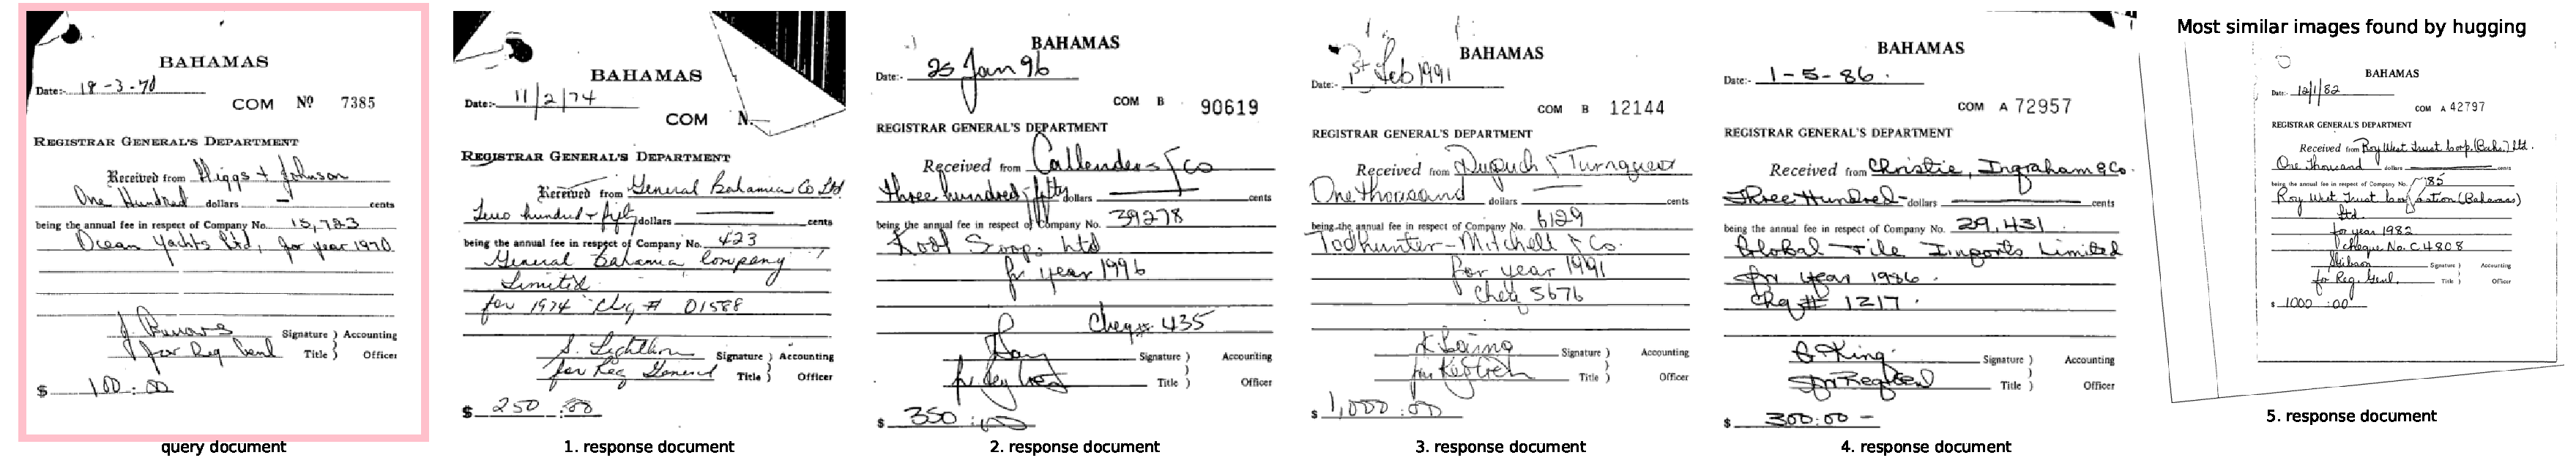
\includegraphics[width=1\textwidth]{images/query_results/4542b223317eba23e4bda3e1536d61c8e2d2890a6439830ca8c62650bc1aac70/Most_similar_images_found_by_hugging.pdf}
        \caption{\ac{sbert}}
        \label{fig:good_query_resp_sbert}
    \end{subfigure}

\caption[Qualitative comparison of query responses]{Qualitative comparison of query responses.
The majority of the query document consists of handwritten text.
The results of the \ac{tfidf} model are not very similar to the query document and thus, are considered to be of poor quality.
The other models, for example \ac{sbert}, produce results which are more similar to the query document.
}
\label{fig:comp_query_resp}
\end{figure}



% investigate certain images
any images which produce unusual results?